\section{Implementation and Numerical Results}
\label{sec:64results}

\minitoc[-3mm]{73mm}{5}

\noindent
In this final section of the chapter,
we study optimal results of the test scenarios and
analyze interpolation errors and optimization results
for topology optimization with B-spline surrogates on sparse grids.



\subsection{Implementation}
\label{sec:641implementation}

In the following, for simplicity,
we combine the two functions to be interpolated,
i.e., the Cholesky factor
$\cholfactor\colon \clint{\*0, \*1} \to \real^{6 \times 6}$ and
the micro-cell density $\denscell\colon \clint{\*0, \*1} \to \real$,
to one single objective function
$\*\objfun\colon \clint{\*0, \*1} \to \real^{m+1}$,
from which both functions can be recovered.

\paragraph{Overview of offline and online phase}

Our method is divided into an offline phase and an online phase,
both of which are sketched in \cref{fig:topoOptPhases}.
The offline phase consists of
generating the spatially adaptive sparse grid
$\sgset = \{\gp{\*l_k,\*i_k} \mid k = 1, \dotsc, \ngp\}$,
solving the corresponding micro-problems,
computing the Cholesky factors, and
hierarchizing the Cholesky factor entries and micro-cell densities
to obtain the sparse grid interpolant $\vsgintp$.
Each optimization iteration of the online phase consists of
evaluating the interpolant $\vsgintp$
for each micro-cell parameter $\mcp{j}$ ($j = 1, \dotsc, M$),
reconstructing the elasticity tensor $\etensorcholintp$ from
the Cholesky factors $\cholfactorintp$,%
\footnote{%
  In addition, the partial derivatives
  $\partialdiff{} \etensorcholintp/\partialdiff{} x_t$
  ($t = 1, \dotsc, d$)
  are evaluated using \cref{eq:choleskyFactorDerivative}.
  This is necessary to employ gradient-based optimization.%
}
and solving the macro-problem to retrieve the approximated compliance value
$\complianceintp(\mcp{1}, \dotsc, \mcp{M})$.
The superscript in $\complianceintp$ indicates that
we do not use the exact elasticity tensors $\etensor$
to compute the compliance value,
but rather the reconstructed and interpolated tensors
$\etensorcholintp$.

\begin{figure}
  \tikzset{
    myCircle/.style={
      circle,
      fill=mittelblau!30,
      draw=mittelblau,
      inner sep=0.5mm,
    }
  }%
  \subcaptionbox{%
    Offline phase (without the actual grid generation).%
  }[149mm]{%
    \begin{tikzpicture}
      \node[myCircle] (points) at (0mm,0mm) {%
        $
          \begin{matrix}
            \gp{\*l_1,\*i_1},\\
            \dots,\\
            \gp{\*l_{\ngp},\*i_{\ngp}}
          \end{matrix}
        $%
      };
      \node[myCircle] (elasticityTensors) at (43mm,0mm) {%
        $
          \begin{matrix}
            \etensor(\gp{\*l_1,\*i_1}),\\
            \dots,\\
            \etensor(\gp{\*l_{\ngp},\*i_{\ngp}})
          \end{matrix}
        $%
      };
      \node[myCircle] (choleskyFactors) at (80mm,0mm) {%
        $
          \begin{matrix}
            \cholfactor(\gp{\*l_1,\*i_1}),\\
            \dots,\\
            \cholfactor(\gp{\*l_{\ngp},\*i_{\ngp}})
          \end{matrix}
        $%
      };
      \node[myCircle] (choleskyInterpolant) at (118mm,0mm) {%
        $
          \begin{matrix}
            \cholfactorintp\colon \clint{\*0, \*1}\\
            {} \to \real^{6 \times 6}
          \end{matrix}
        $%
      };
      \draw[->,draw=C0] (points) -- node[above] {%
        \footnotesize{}micro-problem%
      } (elasticityTensors);
      \draw[->,draw=C0] (elasticityTensors) -- node[above] {%
        \footnotesize{}%
        $
          \tr{\cholfactor} \cholfactor = \etensor
        $\vphantom{p}%
      } (choleskyFactors);
      \draw[->,draw=C0] (choleskyFactors) -- node[above] {%
        \footnotesize{}interpolate%
      } (choleskyInterpolant);
    \end{tikzpicture}%
  }%
  \\[2mm]%
  \subcaptionbox{%
    Online phase (one iteration of the optimizer).%
  }[149mm]{%
    \begin{tikzpicture}
      \node[myCircle] (points) at (0mm,0mm) {%
        $
          \begin{matrix}
            \mcp{1},\\
            \dots,\\
            \mcp{M}
          \end{matrix}
        $%
      };
      \node[myCircle] (choleskyFactors) at (34mm,0mm) {%
        $
          \begin{matrix}
            \cholfactorintp(\mcp{1}),\\
            \dots,\\
            \cholfactorintp(\mcp{M})
          \end{matrix}
        $%
      };
      \node[myCircle] (elasticityTensors) at (83mm,0mm) {%
        $
          \begin{matrix}
            \etensorcholintp(\mcp{1}),\\
            \dots,\\
            \etensorcholintp(\mcp{M})
          \end{matrix}
        $%
      };
      \node[myCircle] (complianceValue) at (129.5mm,0mm) {%
        $
          \begin{matrix}
            \complianceintp(\mcp{1},\\
            \dotsc,\\
            \mcp{M})
          \end{matrix}
        $%
      };
      \draw[->,draw=C0] (points) -- node[above] {%
        \footnotesize{}evaluate\vphantom{p}%
      } (choleskyFactors);
      \draw[->,draw=C0] (choleskyFactors) -- node[above] {%
        \footnotesize{}%
        $
          \etensorcholintp
          = \tr{(\cholfactorintp)} \cholfactorintp
        $\vphantom{p}%
      } (elasticityTensors);
      \draw[->,draw=C0] (elasticityTensors) -- node[above] {%
        \footnotesize{}macro-problem%
      } (complianceValue);
    \end{tikzpicture}%
  }%
  \caption[Offline and online phase for topology optimization]{%
    Offline and online phase for topology optimization.
    The interpolation of the
    micro-cell density $\denscell$ with $\denscellintp$
    (see \cref{sec:622BSplines}) has been omitted for brevity.%
  }%
  \label{fig:topoOptPhases}%
\end{figure}

\paragraph{Generation of spatially adaptive sparse grids}

We use the classical surplus-based refinement criterion
(see, e.g., \cite{Pflueger10Spatially})
as shown in \cref{alg:topoOptGridGeneration}
to generate the spatially adaptive sparse grids.
The difference to common surrogate settings is that the objective function
$\*f\colon \clint{\*0, \*1} \to \real^{m+1}$ is vector-valued.
As the entries of $\cholfactor$ cannot be evaluated individually,
the adaptivity criterion has to consider all entries at once
to avoid performing unnecessary evaluations.
We use the surpluses in the piecewise linear hierarchical basis,
as their absolute values correlate with the second mixed derivative
of the objective function due to \cref{eq:surplusIntegral}.
The surpluses are combined using the formula
$\beta_k \ceq \tr{\*c} \vabs{\vsurplus_{\*l_k,\*i_k}}$
(with entry-wise absolute value) and the
points with largest $\beta_k$ are refined.

\begin{algorithm}
  \begin{algorithmic}[1]
    \Function{$\sgset = \texttt{offlinePhase}$}{%
      $\*\objfun$, $n$, $b$, $\*c$, $l_{\max}$, $\refinetol$,
      $\ngp_{\mathrm{refine}}$%
    }
      \State{$\sgset \gets \coarseregsgset{n}{d}{b}$}
      \Comment{initial regular sparse grid}%
      \While{\True}
        \State{$\ngp \gets \setsize{\sgset}$}
        \Comment{number of grid points}%
        \State{%
          Let $(\vsurplus_{\*l_{k'},\*i_{k'}})_{k' = 1, \dotsc, \ngp}$
          satisfy $
            \fa{k = 1, \dotsc, \ngp}{
              \sum_{k'=1}^{\ngp} \vsurplus_{\*l_{k'},\*i_{k'}}
              \bspl{\*l_{k'},\*i_{k'}}{1}(\gp{\*l_k,\*i_k})
              = \*\objfun(\gp{\*l_k,\*i_k})
            }
          $%
        }
        \ForOneLine{$k = 1, \dotsc, \ngp$}{%
          $\beta_k \gets \tr{\*c} \vabs{\vsurplus_{\*l_k,\*i_k}}$%
        }
        \Comment{combine surpluses to a scalar value}%
        \State{%
          $
            \liset^\ast \gets \{
              k = 1, \dotsc, \ngp \mid
              \ex{\gp{\*l,\*i} \notin \sgset}{
                \gp{\*l_k,\*i_k} \to \gp{\*l,\*i}
              },\,
              \norm[\infty]{\*l_k} < l_{\max},\,
              \abs{\beta_k} > \refinetol
            \}
          $%
        }
        \IfOneLine{$\liset^\ast = \emptyset$}{\Break{}}
        \Comment{stop when there are no refinable grid points left}%
        \State{%
          Refine $\le \ngp_{\mathrm{refine}}$ of the points
          $\{\gp{\*l_k,\*i_k} \in \sgset \mid k \in \liset^\ast\}$
          with largest $\beta_k$%
        }
      \EndWhile{}
    \EndFunction{}
  \end{algorithmic}
  \caption[%
    Generation of spatially adaptive sparse grids for topology optimization%
  ]{%
    Generation of spatially adaptive sparse grids for topology optimization.
    Inputs are
    the objective function $\*f\colon \clint{\*0, \*1} \to \real^{m+1}$
    (combination of the Cholesky factor of the elasticity tensor and
    the micro-cell density),
    the level $n \ge d$ and boundary parameter $b \in \nat$ of the
    initial regular sparse grid,
    the vector $\*c \in \real^{m+1}$ of coefficients with which the
    absolute values of the entries of the surpluses are combined,
    the maximal level $l_{\max} \in \nat$,
    the refinement threshold $\refinetol \in \posreal$, and
    the number $\ngp_{\mathrm{refine}} \in \nat$ of points to refine
    in each iteration.
    Output is the spatially adaptive sparse grid $\sgset$.%
  }%
  \label{alg:topoOptGridGeneration}%
\end{algorithm}

\paragraph{Parameter bounds}

In the micro-cell models presented in \cref{sec:631models},
extreme micro-cell parameters near zero or one may cause problems
with the resulting elasticity tensors.
For instance, many elasticity tensor entries corresponding to
the 2D cross model are discontinuous near the lines $x_1 = 1$ or $x_2 = 1$
\multicite{Huebner14Mehrdimensionale,Valentin14Hierarchische}.
This is due to the fact that the micro-cell is completely filled with material
on these lines,
independent of the other micro-cell parameter.
Similar issues occur for the other models and the shearing angles.
Hence, we have to restrict the range of the feasible micro-cell parameters,
i.e., the sparse grid points
$\*x = \gp{\*l_k,\*i_k}$ are still defined on the unit hyper-cube
$\clint{\*0, \*1}$,
but the actual micro-cell parameters $\xscaled$ are retrieved by an
affine transformation $\xscaled \ceq \*a + (\*b - \*a) \*x$.
For the models in \cref{sec:631models},
we restrict the bar widths to $\clint{0.01, 0.99}$ and
the shearing angles to $\clint{-0.35\pi, 0.35\pi}$.

\paragraph{Software, algorithms, and domain discretization}

The micro-problems and macro-problems were solved with the
\fem software package CFS++ \cite{Kaltenbacher10Advanced}.%
\footnote{%
  \url{http://www.lse.uni-erlangen.de/cfs/}%
}
The micro-prob\-lems were discretized by dividing the micro-cells into
$128 \times 128 = \num{16384}$ elements (models in two dimensions) or
$16 \times 16 \times 16 = \num{4096}$ elements (models in three dimensions).
The macro-domains $\objdomain$ were discretized using
32 macro-cells per meter in the 2D cantilever scenario
(i.e., $64 \times 32 = \num{2048}$ cells),
20 macro-cells per meter in the 3D cantilever scenario
(i.e., $20 \times 20 \times 20 = \num{8000}$ cells), and
10 macro-cells per meter in the other scenarios
(i.e.,
\num{1600} cells for the 2D L-shape and
\num{4000} cells for the 3D center-load).
The generation of the sparse grids (offline phase) was done via a MATLAB code,
while the evaluation of the interpolants (online phase) was performed
by the sparse grid toolbox \sgpp \cite{Pflueger10Spatially}.%
\footnote{%
  \url{http://sgpp.sparsegrids.org/}%
}
For the solution of the emerging optimization problems,
a sequential quadratic programming method was employed
(see \cref{sec:513gradientBasedConstrained}).



\subsection{Error Sources}
\label{sec:642errorSources}

There are multiple sources that contribute to the numerical error
of our method:

\begin{enumerate}[label=E\arabic*.,ref=E\arabic*,leftmargin=2.7em]
  \item
  \label{item:topoOptErrorMicro}
  Discretization of the micro-problem
  (i.e., the elasticity tensors $\etensor$ are inaccurate)
  
  \item
  \label{item:topoOptErrorInterpolation}
  Sparse grid interpolation
  (i.e., $\etensorintp \not= \etensor$)
  
  \item
  \label{item:topoOptErrorCholesky}
  Reconstruction of elasticity tensors with Cholesky factors
  (i.e., $\etensorcholintp \not= \etensorintp$)
  
  \item
  \label{item:topoOptErrorMacro}
  Discretization of the macro-problem
  (i.e., the compliance $\compliance$ is inaccurate)
  
  \item
  \label{item:topoOptErrorOptimization}
  Optimization
  (i.e., the minimum found by the optimizer is inaccurate or not global)
  
  \item
  \label{item:topoOptErrorRounding}
  Floating-point rounding errors
  (i.e., arithmetical operations are inaccurate)
\end{enumerate}

\noindent
\ref{item:topoOptErrorRounding}-type errors are always present and
will not be analyzed in this chapter.
Errors of type \ref{item:topoOptErrorMicro} and \ref{item:topoOptErrorMacro}
are intrinsic to the homogenization approach
and will not be discussed here either.
The optimization error \ref{item:topoOptErrorOptimization}
has already been discussed in \cref{sec:542optimization}
for explicit test functions.
Therefore, in the remainder of this chapter,
we will focus on the analysis of the errors of types
\ref{item:topoOptErrorInterpolation} and \ref{item:topoOptErrorCholesky},
since the interpolation of Cholesky factors is the
major new contribution to this application.



\subsection{Interpolation Error}
\label{sec:643interpolation}

\paragraph{Spectral interpolation error measure}

For the interpolation error \ref{item:topoOptErrorInterpolation} and
the Cholesky factorization error \ref{item:topoOptErrorCholesky},
we cannot simply take the absolute value of the difference
of the objective function $\*\objfun\colon \clint{\*0, \*1} \to \real^{m+1}$
and its surrogate $\vsgintp$, since both are vector-valued.
As the micro-cell density $\denscell$
is not affected by the Cholesky factorization,
we consider only the elasticity tensor
$\etensor\colon \clint{\*0, \*1} \to \real^{6 \times 6}$ and
its surrogate
$\etensorcholintp\colon \clint{\*0, \*1} \to \real^{6 \times 6}$
obtained by Cholesky factorization.
To retrieve a scalar error measure,
we use the spectral norm
\begin{equation}
  \norm[2]{\etensor(\*x) - \etensorcholintp(\*x)},\quad
  \*x \in \clint{\*0, \*1},
\end{equation}
i.e., the largest absolute eigenvalue of
$\etensor(\*x) - \etensorcholintp(\*x)$.
However, the choice of the norm is arbitrary,
as all matrix norms on $\real^{6 \times 6}$ are equivalent to each other.

\paragraph{Pointwise spectral interpolation error}

\Cref{fig:topoOptInterpolationErrorPointwise}
shows the pointwise spectral interpolation error for the 2D cross model
and the corresponding spatially adaptive sparse grid
generated with the refinement algorithm as explained in
\cref{sec:641implementation}.
The above-mentioned discontinuity of elasticity tensor entries
near $x_1 = 1$ or $x_2 = 1$
is most severe near the corners $\*x \in \{(0, 1), (1, 0)\}$
(cf.\ \cref{fig:cholesky}),
as some entries vanish if one of the micro-cell bars has zero width.
Hence, most points are placed near these singularity corners.

\begin{figure}
  \subcaptionbox{%
    $\norm[2]{\etensor(\*x) - \etensorintp(\*x)}$%
    \label{fig:topoOptInterpolationErrorPointwise_1}%
  }[63mm]{%
    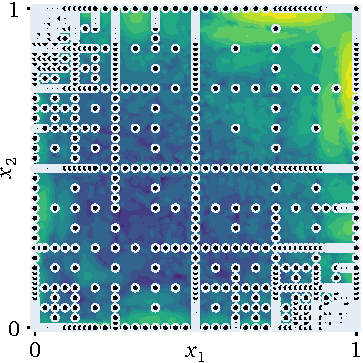
\includegraphics{topoOptInterpolationPointwise_1}%
  }%
  \hspace{3mm}%
  \subcaptionbox{%
    $\norm[2]{\etensor(\*x) - \etensorcholintp(\*x)}$%
    \label{fig:topoOptInterpolationErrorPointwise_2}%
  }[63mm]{%
    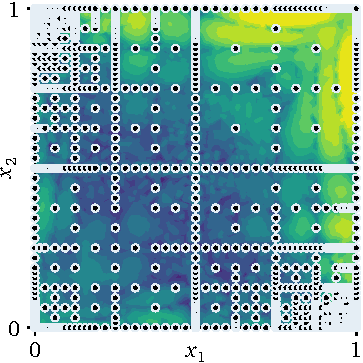
\includegraphics{topoOptInterpolationPointwise_2}%
  }%
  \hfill%
  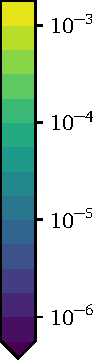
\includegraphics{topoOptInterpolationPointwise_3}%
  \caption[Pointwise spectral interpolation error for the 2D cross model]{%
    Pointwise spectral interpolation error for the 2D cross model and
    cubic B-splines on
    $\ngp = 1320$ spatially adaptive sparse grid points \emph{(dots)} for
    the direct elasticity tensor interpolation \emph{(left)} and
    the Cholesky factor interpolation \emph{(right).}%
  }%
  \label{fig:topoOptInterpolationErrorPointwise}%
\end{figure}

The left plot (\cref{fig:topoOptInterpolationErrorPointwise_1})
shows the spectral interpolation error
$\norm[2]{\etensor(\*x) - \etensorintp(\*x)}$
of the direct elasticity tensor interpolant without Cholesky factorization
(i.e., error \ref{item:topoOptErrorInterpolation}).
The maximum error is \num{1.2e-3},
which is attained near the critical lines $x_1 = 1$ or $x_2 = 1$.
Note that the mean error over the whole domain $\clint{\*0, \*1}$
is only \num{4.5e-5}.
In the right plot (\cref{fig:topoOptInterpolationErrorPointwise_2}),
the picture changes slightly when looking at the spectral interpolation error
$\norm[2]{\etensor(\*x) - \etensorcholintp(\*x)}$
of the elasticity tensor resulting from Cholesky factorization
(i.e., errors \ref{item:topoOptErrorInterpolation} and
\ref{item:topoOptErrorCholesky} combined).
The maximum error becomes \num{3.4e-3},
while the mean error increases to \num{1.1e-4}.
We conclude that the Cholesky factorization leads to an increase
of interpolation errors by only less than half an order of magnitude.

\paragraph{Convergence of spectral interpolation error}

\Cref{fig:topoOptInterpolationErrorBasisFunctions_1} shows
the convergence of the relative $\Ltwo$ spectral interpolation errors
\begin{equation}
  \error^{\sparse} \ceq
  \frac{
    \normLtwoscaled{
      \vphantom{\big(}
      \norm[2]{\etensor({\cdot}) - \etensorintp({\cdot})}
    }
  }{
    \normLtwoscaled{
      \vphantom{\big(}
      \norm[2]{\etensor({\cdot})}
    }
  }, \qquad
  \error^{\chol,\sparse} \ceq
  \frac{
    \normLtwoscaled{
      \vphantom{\big(}
      \norm[2]{\etensor({\cdot}) - \etensorcholintp({\cdot})}
    }
  }{
    \normLtwoscaled{
      \vphantom{\big(}
      \norm[2]{\etensor({\cdot})}
    }
  }
\end{equation}
for the 2D cross model, i.e.,
the relative $\Ltwo$ error of the functions depicted in
\cref{fig:topoOptInterpolationErrorPointwise}.
Relative errors of \SI{1}{\permille} are already obtained
for $\ngp = 200$ grid points.
Unfortunately, even for higher B-spline degrees $p > 1$,
the order of convergence is only quadratic
due to the singularities of the elasticity tensor.
This slow convergence does not improve for the other
micro-cell models as shown in
\Cref{fig:topoOptInterpolationErrorBasisFunctions_2}.
In fact, the convergence decelerates even more
as the number of micro-cell parameters increases.
For the 2D sheared cross and 3D cross models with three parameters,
the spatially adaptive sparse grid with $\ngp \approx \num{10000}$ grid points
is able to achieve a relative error of around \SI{3}{\permille}.
However, for the 2D sheared framed cross and 3D sheared cross models
with five parameters, only errors of about \SI{5}{\percent} are reached
for the same grid size.

\begin{figure}
  \hspace*{5mm}%
  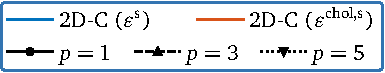
\includegraphics{topoOptInterpolation_3}%
  \hfill%
  \raisebox{0.5mm}{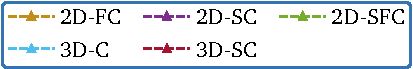
\includegraphics{topoOptInterpolation_4}}%
  \\[2mm]%
  \subcaptionbox{%
    $\error^{\sparse}$ \emph{\textcolor{C0}{(blue)}} and
    $\error^{\chol,\sparse}$ \emph{\textcolor{C1}{(red)}}
    for the 2D cross model and different degrees.%
    \label{fig:topoOptInterpolationErrorBasisFunctions_1}%
  }[72mm]{%
    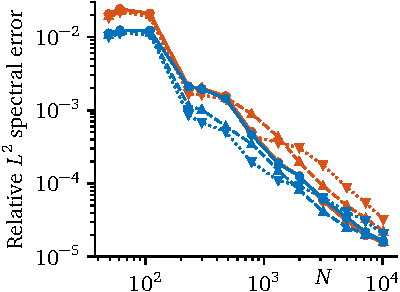
\includegraphics{topoOptInterpolation_1}%
  }%
  \hfill%
  \subcaptionbox{%
    $\error^{\chol,\sparse}$
    for the other models and $p = 3$.%
    \label{fig:topoOptInterpolationErrorBasisFunctions_2}%
  }[72mm]{%
    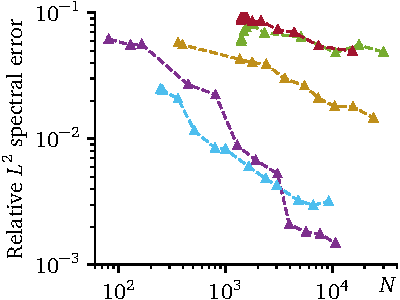
\includegraphics{topoOptInterpolation_2}%
  }%
  \caption[Convergence of relative $L^2$ spectral interpolation errors]{%
    Convergence of relative $\Ltwo$ spectral interpolation errors
    over the increasing number $\ngp$ of spatially adaptive grid points
    (i.e., decreasing threshold $\refinetol$)
    for the 2D cross model without or with Cholesky factor interpolation
    and different degrees $p$ \emph{(left)} and
    for the other models and cubic degree \emph{(right)}.%
  }%
  \label{fig:topoOptInterpolationErrorBasisFunctions}%
\end{figure}



\subsection{Optimal Compliance Values and Structures}
\label{sec:644optimization}

\paragraph{Optimal compliance values for different micro-cell models}

In the following, we use for each micro-cell model
a specific spatially adaptive sparse grid with around \num{10000} points.
The exact grid sizes and other details about the employed sparse grids
can be found in \cref{tbl:topoOptModels}
(located in \cref{chap:a30topoOptDetails}).
For hierarchical cubic B-splines ($p = 3$),
\cref{tbl:topoOptResultsModels} lists the
compliance values $\compliance(\mcpoptappr{1}, \dotsc, \mcpoptappr{M})$
for each of the four scenarios
and the corresponding possible micro-cell models,
where $(\mcpoptappr{1}, \dotsc, \mcpoptappr{M}) \in (\real^d)^M$
is the micro-cell parameter combination that is returned by the optimizer.%
\footnote{%
  Note that this true compliance value differs from the
  approximated value
  $\complianceintp(\mcpoptappr{1}, \dotsc, \mcpoptappr{M})$,
  which the optimizer reports as the optimal objective function value.%
}
It is obvious that more complicated micro-cell models
lead to lower (better) compliance values,
as they are a generalization of the simple models.
For instance, the 2D cross is a special case of
the 2D framed cross, the 2D sheared cross, and the 2D sheared framed cross.
By choosing the respectively best model for each scenario,
we are able to decrease the compliance value
(and, hence, increase the stability of the resulting structure)
by \SI{9.6}{\percent} in the 2D cantilever scenario,
by \SI{7.7}{\percent} in the 2D L-shape scenario,
by \SI{34}{\percent} in the 3D cantilever scenario, and
by \SI{73}{\percent} in the 3D center-load scenario.
In general, this motivates the usage of more complicated micro-cell models,
which cannot be computationally handled with
conventional full grid interpolation methods.
Consequently, sparse grids or similar methods have to be used.

\begin{table}
  \setnumberoftableheaderrows{1}%
  \begin{tabular}{%
    >{\kern\tabcolsep}=l<{\kern5mm}*{6}{+c}<{\kern\tabcolsep}%
  }
    \toprulec
    \headerrow
    Scenario&       2D-C&   2D-FC&  2D-SC&           2D-SFC& 3D-C&   3D-SC\\
    \midrulec
    2D cantilever&  74.974& 70.816& \textbf{67.809}& 68.602& ---&    ---\\
    2D L-shape&     183.68& 177.51& \textbf{169.60}& 174.55& ---&    ---\\
    \midrulec
    3D cantilever&  ---&    ---&    ---&             ---&    247.60& \textbf{162.59}\\
    3D center-load& ---&    ---&    ---&             ---&    169.27& \textbf{46.171}\\
    \bottomrulec
  \end{tabular}
  \caption[Optimal compliance values for different micro-cell models]{%
    Optimal compliance values for the different scenarios
    and micro-cell models using cubic B-splines
    (spatially adaptive grids with around \num{10000} points).
    The entries highlighted in \textbf{bold face} indicate the best choice
    of micro-cell models for a given scenario.
    More details can be found in \cref{tbl:topoOptResultsDetailed}.%
  }%
  \label{tbl:topoOptResultsModels}%
\end{table}

\paragraph{Corresponding optimal structures}

The corresponding optimal structures are shown in
\cref{fig:topoOptStructure2DCantilever} for the 2D cantilever scenario
and, for reasons of space, in \cref{chap:a30topoOptDetails} in
\cref{fig:topoOptStructure2DLShape,fig:topoOptStructure3D}
for the other three scenarios.
Of course, the periodic micro-cell structures cannot be plotted directly,
as the micro-cells are infinitesimally small.
Therefore, the figures show for each macro-cell only
one single large micro-cell.

\begin{figure}
  \subcaptionbox{%
    2D cross%
  }[72mm]{%
    
\includegraphics{topoOptStructure2D_1}%
  }%
  \hfill%
  \subcaptionbox{%
    2D framed cross%
  }[72mm]{%
    
\includegraphics{topoOptStructure2D_3}%
  }%
  \\[2mm]%
  \subcaptionbox{%
    2D sheared cross%
  }[72mm]{%
    
\includegraphics{topoOptStructure2D_5}%
  }%
  \hfill%
  \subcaptionbox{%
    2D sheared framed cross%
  }[72mm]{%
    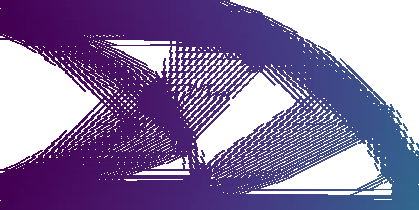
\includegraphics{topoOptStructure2D_7}%
  }%
  \caption[Optimal structures in the 2D cantilever scenario]{%
    Topologically optimal structures in the 2D cantilever scenario
    for different micro-cell models using cubic B-splines
    (spatially adaptive grids with around \num{10000} points).
    The colors indicate the length of the displacement,
    where dark regions correspond to weak displacements and
    bright regions to strong displacements.
    The color map is the same as in
    \cref{fig:topoOptStructure2DLShape}.
    Only bars with widths $\ge 0.1$ are shown.
    More details can be found in \cref{tbl:topoOptResultsDetailed}.%
  }%
  \label{fig:topoOptStructure2DCantilever}%
\end{figure}

Two effects can be seen in the plots of the optimal structures:
First, the simpler models are not able to direct the emerging forces at
arbitrary angles.
For example, the 2D framed cross model strongly prefers
angles of \ang{45}, which results in structures that are not as stable
as they could be.
The 2D sheared cross and 2D sheared framed cross models
are considerably more flexible, allowing
internal forces to act at almost arbitrary angles.
Second, the sheared micro-cell models use the available
material volume more efficiently than the cross model.
This is most striking in the 3D case (see \cref{fig:topoOptStructure3D}),
where it seems that the sheared cross structures
use more volume than the simple cross structures,
although the structures spend exactly the same amount of material volume.
The reason is that for the cross model, both bars
have to be used in order to connect the macro-cell to its neighbors.
For the sheared cross model, a shearing of the vertical bar suffices,
and we save volume by not using the horizontal bar.
Both of these effects explain the significantly lower compliance
values for the sheared micro-cell models.

\paragraph{Comparison to the direct solution}

B-splines on sparse grids lead to a drastic reduction in computation time.
Solving the 2D cantilever scenario with the best-placed sheared cross model
would take 453 days with
exact elasticity tensor evaluations (i.e., without surrogates),
assuming the same number of iterations as for the surrogate tensor case
and sequential computation of the elasticity tensors.
This estimate does not account for approximating the missing derivatives
of the elasticity tensor.
If we incorporate this and use 100 parallel processes,
we still need weeks for the solution.
In contrast, the computation time using our sparse grid surrogates
is a matter of minutes or hours at most,
resulting in speedups of around 200.
This is excluding the time for the offline phase,
which is in the range of hours, but which has to be spent only once,
as the resulting grid can be reused for different scenarios.

\vspace{2em}

\paragraph{Optimality-interpolation gaps}

\begin{figure}
  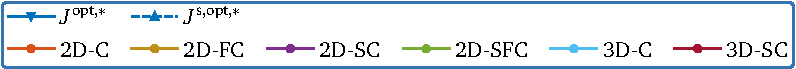
\includegraphics{topoOptOptimalityGap_3}%
  \\[2mm]%
  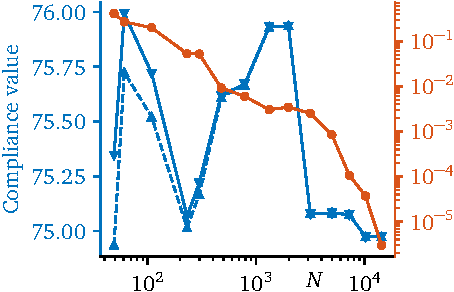
\includegraphics{topoOptOptimalityGap_1}%
  \hfill%
  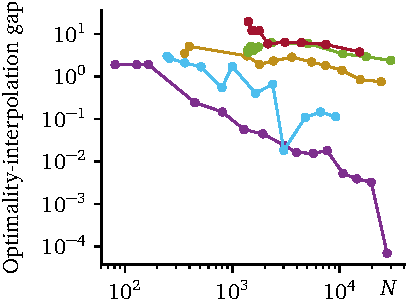
\includegraphics{topoOptOptimalityGap_2}%
  \caption[Convergence of the optimality-interpolation gap]{%
    Convergence of the optimality-interpolation gap
    $\abs{\compliance[\opt,\ast] - \complianceintp[\opt,\ast]}$
    for the 2D/3D cantilever scenario
    and different micro-cell models using cubic B-splines ($p = 3$).
    The left plot additionally shows
    $\compliance[\opt,\ast]
    \ceq \compliance(\mcpoptappr{1}, \dotsc, \mcpoptappr{M})$ and
    $\complianceintp[\opt,\ast]
    \ceq \complianceintp(\mcpoptappr{1}, \dotsc, \mcpoptappr{M})$
    for the 2D cross model.%
  }%
  \label{fig:topoOptOptimalityGap}%
\end{figure}

Ideally, we would measure the true optimality gap
\begin{equation}
  \label{eq:topoOptOptimalityGapTrue}
  \compliance(\mcpoptappr{1}, \dotsc, \mcpoptappr{M}) -
  \compliance(\mcpopt{1}, \dotsc, \mcpopt{M}),
\end{equation}
cf.\ error \ref{item:topoOptErrorOptimization}.
Unfortunately, the true optimum
$(\mcpopt{1}, \dotsc, \mcpopt{M})$ could not be computed:
Apart from the time issue mentioned above,
oscillations in the elasticity tensor evaluation and
errors stemming from types
\ref{item:topoOptErrorMicro} and \ref{item:topoOptErrorRounding}
reliably led to optimizer crashes as it ran into discontinuities,
which are smoothed out when using B-spline surrogates.
However, as in \cref{fig:topoOptOptimalityGap},
we can at least calculate the \term{optimality-interpolation gap}
\begin{equation}
  \label{eq:topoOptOptimalityGapPseudo}
  \abs{
    \compliance(\mcpoptappr{1}, \dotsc, \mcpoptappr{M}) -
    \complianceintp(\mcpoptappr{1}, \dotsc, \mcpoptappr{M})
  }
\end{equation}
between the actual compliance value
and the approximated, reported compliance value.
This gap does not constitute any kind of bound on the true optimality gap;
however, the idea is that
as the interpolation error converges to zero,
the optimality-interpolation gap should converge to zero, too.

\pagebreak

\Cref{fig:topoOptOptimalityGap} (left) shows that for the 2D cross model,
the optimizer reports compliance values that are smaller than in reality
($\complianceintp[\opt,\ast]$ vs. $\compliance[\opt,\ast]$).
However, the difference steadily converges to zero.
This is similar for the other micro-cell model as shown in the
right part of \cref{fig:topoOptOptimalityGap},
although the convergence is much slower due to the
higher number $d$ of micro-cell parameters.

\paragraph{Optimal compliance values for different B-spline degrees}

Finally, to study the effect of the B-spline degree on the
optimization performance,
\cref{tbl:topoOptResultsDegrees} lists the compliance values
for the degrees $p = 1, 3, 5$ and the 2D/3D cross and sheared cross
micro-cell models.
In the two-dimensional scenarios,
higher-order B-splines decrease the compliance value
by up to \SI{9}{\percent}.
In the three-dimensional scenarios,
higher-order B-splines may perform worse than the piecewise linear
functions ($p = 1$).
(However, as indicated in \cref{tbl:topoOptResultsDegrees},
all optimization runs with piecewise linear functions
terminated prematurely due to numerical difficulties with the
discontinuous derivatives.)
It may be suspected that if we used micro-cell models with
less prominent discontinuities (i.e., ``smoother'' elasticity tensors),
the advantage of higher-order B-splines would be more visible.
All in all, the application of topology optimization underlines
that good interpolation (and thus a good quality of the surrogate)
is key to good optimization results.

\begin{table}
  \setnumberoftableheaderrows{2}%
  \begin{tabular}{%
      >{\kern\tabcolsep}=l<{\kern5mm}*{3}{+c}%
      <{\kern5mm}*{3}{+c}<{\kern\tabcolsep}%
    }
    \toprulec
    \headerrow
    &
    \multicolumn{3}{c}{\hspace*{-12pt}2D/3D cross}&
    \multicolumn{3}{c}{\hspace*{-6pt}2D/3D sheared cross}\\
    \headerrow
    Scenario&       $p = 1$&         $p = 3$&         $p = 5$&          $p = 1$&                $p = 3$&         $p = 5$\\
    \midrulec
    2D cantilever&  \emph{82.365}&   \textbf{74.974}& 76.070&           \emph{68.889}&          \textbf{67.809}& 68.018\\
    2D L-shape&     \emph{193.83}&   \textbf{183.68}& 183.70&           \emph{169.85}&          169.60&          \textbf{169.60}\\
    \midrulec
    3D cantilever&  \emph{249.75}&   247.60&          \textbf{247.33}&  \emph{\textbf{148.72}}& 162.59&          152.34\\
    3D center-load& \textbf{162.68}& 169.27&          163.94&           \emph{\textbf{45.713}}& 46.171&          47.074\\
    \bottomrulec
  \end{tabular}
  \caption[Optimal compliance values for different B-spline degrees]{%
    Optimal compliance values for the different scenarios
    and B-spline degrees using the 2D/3D cross micro-cell model \emph{(left)}
    and the 2D/3D sheared cross micro-cell model \emph{(right).}
    The spatially adaptive sparse grids are the same as in
    \cref{tbl:topoOptResultsModels}.
    The entries highlighted in \textbf{bold face} indicate the best choice
    of B-spline degree for a given scenario and micro-cell model.
    Optimization runs of entries marked as \emph{italic}
    terminated prior to success due to numerical difficulties.%
  }%
  \label{tbl:topoOptResultsDegrees}%
\end{table}
